\documentclass[10pt]{beamer} %
\usetheme{CambridgeUS}
% \usecolortheme{seahorse}
\usecolortheme{orchid}
% \usepackage[latin1]{inputenc}
\usefonttheme{professionalfonts}
\usepackage{times}
%\usepackage{tikz}
\usepackage{tikz}
\usepackage{pgfplots}
\pgfplotsset{compat=1.18} % Ensures compatibility for the plot
\usepackage{amsmath}
\usepackage{verbatim}
\usepackage{graphicx}
\usepackage{multicol}
%\usetikzlibrary{arrows,shapes}
\setlength{\tabcolsep}{20pt}
\renewcommand{\arraystretch}{1.5}

\usepackage{amsmath,amssymb,amsfonts}
\usepackage{hyperref}
\usepackage{textcomp}
\usepackage[english]{babel}
\usepackage{times}
% \usepackage[T1]{fontenc}

\usepackage{xcolor}
\usepackage{color, colortbl}
\usepackage{multirow}

%\usepackage{beamerthemesplit}
%\usetheme{Warsaw}
\setbeamertemplate{footline}[frame number]
%\usefonttheme{structurebold}
%\usefonttheme[onlymath]{serif}
%\usefonttheme{serif}
\usepackage{pgf}
\usepackage{amsmath,amssymb}
% \usepackage{inputenc}
%\usepackage[latin1]{inputenc}
\usepackage[english]{babel}
\usepackage{times}
\usepackage{hyperref}
\usepackage{colortbl}
\usepackage{helvet}
\usepackage{booktabs}
\usepackage{multirow}

\usepackage{tikz}
\usetikzlibrary{arrows,shapes,trees, positioning}
\usepackage{graphics}
\usepackage{color}

\pgfdeclarelayer{background}
\pgfdeclarelayer{foreground}
\pgfsetlayers{background,main,foreground}


%\usepackage[dvipsnames]{xcolor}
%\graphicspath{{images/}}
%\renewcommand{\baselinestretch}{1.5}
% \usepackage[utf8]{inputenc} % allow utf-8 input
% \usepackage[T1]{fontenc}    % use 8-bit T1 fonts
%\usepackage{listings}
%\usepackage{hyperref}       % hyperlinks
%\usepackage{url}            % simple URL typesetting
%\usepackage{booktabs}       % professional-quality tables
%\usepackage{amsfonts}       % blackboard math symbols
%\usepackage{nicefrac}       % compact symbols for 1/2, etc.
%\usepackage{microtype}      % microtypography
%\usepackage{lipsum}
% \usepackage{fancyhdr}       % header
%\usepackage{graphicx}       % graphics
%\usepackage{caption}
%\usepackage{subcaption}
%\usepackage[dvipsnames]{xcolor}
%\usepackage{cite}
%\usepackage{epsfig}
%\usepackage{textcomp}
%\usepackage{bm}
%
%\usepackage{algorithm}
%\usepackage{algorithmic}
%\usepackage{dsfont}
%\usepackage{appendixnumberbeamer}
%Header
% \pagestyle{fancy}
% \thispagestyle{empty}
% \rhead{ \textit{ }} 
% \setlength{\tabcolsep}{15pt}


\newcommand{\defn}{\textcolor{red}{Def:~}}
%\AtBeginEnvironment{frame}{\setcounter{myc}{0}}
\newcounter{myc}[section]%framenumber]
\newcommand{\expl}{\textcolor{blue}{\stepcounter{myc}Example~\arabic{myc}:~}}
\newcommand{\theo}{\textcolor{brown}{Theorem:~}}
\newcommand{\coro}{\textcolor{brown}{Corollary:~}}
\newcommand{\remark}{\textcolor{brown}{Remark:~}}
\newcommand{\sam}{\mathcal{S}}
\newcommand{\sig}{\mathcal{F}}
\newcommand{\R}{\mathbb{R}}
\newcommand{\bg}{\boldsymbol{g}}
\newcommand{\bX}{\boldsymbol{X}}
\newcommand{\bx}{\boldsymbol{x}}
\newcommand{\bY}{\boldsymbol{Y}}
\newcommand{\by}{\boldsymbol{y}}
\newcommand{\bt}{\boldsymbol{t}}
\newcommand{\bu}{\boldsymbol{u}}
\newcommand{\bmu}{\boldsymbol{\mu}}
\newcommand{\mc}{\{X_n:n\geq0\}}


\title[]{Statistical Inference and Multivariate Analysis (MA324)}
\subtitle{\textsc{Lecture Slides}\\Topic 04\\ Multivariate Analysis}
\date{Jan-May 2026}


\graphicspath{{plots/}}

\begin{document}

% ===================================================================== Frame : Title Page
\thispagestyle{empty}
\maketitle

\begin{frame}
   \frametitle{Principal Component Analysis}
   \begin{itemize}
      \item Concerned with explaining the variance-covariance structure of a set
         of variables through a few linear combinations of these variables. 
         \vspace{0.45cm}
      \item Objectives
         \vspace{0.45cm}
         \begin{itemize}
            \item Data Reduction.
               \vspace{0.25cm}
            \item Interpretation.
         \end{itemize}
         \vspace{0.45cm}
      \item Serves as intermediate steps in a larger study (Multiple Linear
         Regression, Cluster Analysis).
         \vspace{0.45cm}
      \item Wide application areas: including image analysis, finance, health
         sector, cryptography, data-privacy etc. 
   \end{itemize}
\end{frame}

\begin{frame}
   \frametitle{Population Principal Components}
   \begin{itemize}
      \item Let $X_1,X_2,...,X_p$ be $p$-random variables with variance-covariance matrix $\Sigma$.
         \vspace{0.25cm}	
      \item First we want to find a linear combination of
         $\boldsymbol{X}=(X_1,X_2,...,X_p)$, say
         $\boldsymbol{a_{1}'}\boldsymbol{X}$, such that
         $Var(\boldsymbol{a_{1}'}\boldsymbol{X})$ is maximum.
         \vspace{0.25cm}		
      \item Note that
         $Var(\boldsymbol{a_{1}'}\boldsymbol{X})=\boldsymbol{a_{1}'}\Sigma\boldsymbol{a_1}$.
         Now by multiplying $\boldsymbol{a_1}$ by a constant, we can increase
         $\boldsymbol{a_{1}'}\Sigma\boldsymbol{a_1}$ arbitrarily.
         \vspace{0.25cm}
      \item Therefore, a more precise aim is:
         \begin{equation*}
            \operatorname*{max}_{\boldsymbol{a_1}}
            Var(\boldsymbol{a_{1}'}\boldsymbol{X})=\operatorname*{max}_{\boldsymbol{a_1}}
            \boldsymbol{a_{1}'}\Sigma\boldsymbol{a_1},
         \end{equation*}
         subject to $\boldsymbol{a_{1}'}\boldsymbol{a_{1}}=1$
   \end{itemize}	
\end{frame}

\begin{frame}
   \frametitle{}
   \begin{itemize}
      \item Thus, $1^{st}$ principal component = linear combination
         $\boldsymbol{a_{1}'}\boldsymbol{X}$ which maximizes
         $Var(\boldsymbol{a_{1}'}\boldsymbol{X})$ subject to
         $\boldsymbol{a_{1}'}\boldsymbol{a_{1}}=1$
         \vspace{0.25cm}
      \item Next, we want to find another linear cobination, say
         $\boldsymbol{a_{2}'}\boldsymbol{X}$, such that
         $Var(\boldsymbol{a_{2}'}\boldsymbol{X})$ is maximum subject to
         $\boldsymbol{a_{2}'}\boldsymbol{a_2}=1$ and
         $Cov(\boldsymbol{a_{1}'}\boldsymbol{X},\boldsymbol{a_{2}'}\boldsymbol{X})
         = 0$.
         \vspace{0.25cm}
      \item We proceed in the following manner	
         \begin{itemize}
            \item $i^{th}$ principle component = linear combination
               $\boldsymbol{a_{i}'}\boldsymbol{X}$ that maximizes
               $Var(\boldsymbol{a_{i}'}\boldsymbol{X})$ subject to
               $\boldsymbol{a_{i}'}\boldsymbol{a_i}=1$ and
               $Cov(\boldsymbol{a_{k}'}\boldsymbol{X},\boldsymbol{a_{i}'}\boldsymbol{X})
               = 0$ for $k<i$.
         \end{itemize}
         \vspace{0.25cm}
      \item Notice that
         $Cov(\boldsymbol{a_{k}'}\boldsymbol{X},\boldsymbol{a_{i}'}\boldsymbol{X})
         = \boldsymbol{a_{i}'}\Sigma\boldsymbol{a_k}$, and
         $Var(\boldsymbol{a_{i}'}\boldsymbol{X}) =
         \boldsymbol{a_{i}'}\Sigma\boldsymbol{a_i}$.
   \end{itemize}	
\end{frame}


\begin{frame}
   \frametitle{Theorem: Maximization of Quadratic Forms}
   Let $B_{p \times p}$ be a symmetric non-negative definite matrix with
   eigen-values $\lambda_1 \geq \lambda_2 \geq ... \geq \lambda_p \geq 0$ and
   associated normalized eigen-vectors $\boldsymbol{e_1},
   \boldsymbol{e_2},...,\boldsymbol{e_p}$. Then,
   \begin{eqnarray}
      &&	\operatorname*{max}_{\boldsymbol{x} \neq \boldsymbol{0}}
      \frac{\boldsymbol{x}^{'}B\boldsymbol{x}}{\boldsymbol{x}^{'}\boldsymbol{x}}
      = \lambda_1 \left(=
      \frac{\boldsymbol{e_1}^{'}B\boldsymbol{e_1}}{\boldsymbol{e_1}^{'}\boldsymbol{e_1}}
      \right)\ \text{ attained at } \boldsymbol{x}=\boldsymbol{e_1}, \nonumber \\
      && \operatorname*{min}_{\boldsymbol{x} \neq \boldsymbol{0}}
      \frac{\boldsymbol{x}^{'}B\boldsymbol{x}}{\boldsymbol{x}^{'}\boldsymbol{x}} =
      \lambda_p \text{ attained at } \boldsymbol{x}=\boldsymbol{e_p} \nonumber
   \end{eqnarray}	
   Moreover,
   \begin{eqnarray}
      &&	\operatorname*{max}_{\boldsymbol{x} \neq \boldsymbol{0}, \boldsymbol{x}
      \perp \boldsymbol{e_1},...,\boldsymbol{e_{k-1}}}
      \frac{\boldsymbol{x}^{'}B\boldsymbol{x}}{\boldsymbol{x}\boldsymbol{x}^{'}}
      = \lambda_k \text{ attained at } \boldsymbol{x}=\boldsymbol{e_k}, k=1,2,...,p
      \nonumber
   \end{eqnarray}
\end{frame}

\begin{frame}
   \frametitle{Theorem }
   Let $\Sigma_{p \times p}$ be the variance-covariance matrix of
   $\boldsymbol{X}_{p \times 1} = (X_1,...,X_p)$. Let $\Sigma$ have the
   eigen-value-eigen-vector pair
   $(\lambda_1,e_1),(\lambda_2,e_2),...,(\lambda_p,e_p)$ where $\lambda_1 \geq
   \lambda_2 \geq ... \geq \lambda_p \geq 0$. Then the $i^{th}$ principal
   component is given by,
   \begin{equation*}
      Y_i=\boldsymbol{e_i}^{'}\boldsymbol{X},\ \ \ \ i=1,2,...,p.
   \end{equation*}
   With these choices $Var(Y_i)=\lambda_i$ and $Cov(Y_i,Y_j)=0\ for\ i \neq j.$
   Moreover, if some $\lambda_i$ are equal, the choices of $e_i$ are not unique,
   and hence $Y_i$ are not unique.
\end{frame}

\begin{frame}
   \frametitle{Theorem }
   \begin{equation*}
      \sum_{i=1}^p Var(X_i) = \sigma_{11}+\sigma_{22}+...+\sigma_{pp}=tr(\Sigma)
      = \lambda_1+\lambda_2+...+\lambda_p=\sum_{i=1}^p Var(Y_i).
   \end{equation*}
   \vspace{0.5cm}
   \begin{itemize}
      \item Therefore, the proportion of total variance explained by $i^{th}$
         principal component is $\frac{\lambda_i}{\lambda_1+...+\lambda_p}$,
         $i=1,2,...,p$.
         \vspace{0.5cm}
      \item $e_{ik}$ measures the importance of $X_k$ to the $i^{th}$ principal
         component.
         % \vspace{0.5cm}
      % \item Particularly, $e_{ik}$ is proportional to the correlation
      %    coefficient between $Y_i$ and $X_k$. 
   \end{itemize}
\end{frame}

\begin{frame}
   \frametitle{Theorem }
   If $Y_1=\boldsymbol{e_1}^{'}\boldsymbol{X},
   Y_2=\boldsymbol{e_2}^{'}\boldsymbol{X}, \cdots,
   Y_p=\boldsymbol{e_p}^{'}\boldsymbol{X}$ are the principal components
   obtained from the covariance matrix $\Sigma$, then the correlation
   coefficient between the $Y_i$ and $X_k$ is 
   \begin{equation*}
      \rho_{Y_i,X_k} = \frac{e_{ik}\sqrt{\lambda_i}}{\sqrt{\sigma_{kk}}}.
   \end{equation*}
\end{frame}

\begin{frame}
   \frametitle{Principal Components Obtained from Standardized Variables}
   \begin{eqnarray}
      &&	Z_i = \frac{X_i-\mu_i}{\sqrt{\sigma_{ii}}}, i=1,2,...,p \nonumber \\
      &\Leftrightarrow& \boldsymbol{Z} = \begin{pmatrix}
         Z_1\\ . \\ . \\ . \\
         Z_p 
      \end{pmatrix} = V^{-1}(\boldsymbol{X}-\boldsymbol{\mu}),\ where\
      V=diag(\sqrt{\sigma_{11}},\sqrt{\sigma_{22}},...,\sqrt{\sigma_{pp}})
      \nonumber
   \end{eqnarray}
\end{frame}

\begin{frame}
   \begin{itemize}
      \item $Var(\boldsymbol{Z}) = \rho_{p \times p}=\begin{pmatrix}
            \rho_{11}(=1) & . & . & . & \rho_{1p} \\ . & & & & . \\ . & & & & .
            \\ . & & & & . \\ \rho_{p1} & . & . & . & \rho_{pp}(=1)
         \end{pmatrix}$
      \item $\sum_{i=1}^p Var(Y_i) = p$
         \vspace{0.5cm}
      \item Proportion of standardized population variance due to $k^{th}$
         principal component $=\frac{\lambda_k}{p},\ k=1,2,...,p,$ where
         $\lambda_k$'s are the eigen values of $\rho_{p \times p}$.
   \end{itemize}
\end{frame}

\begin{frame}
   \frametitle{Summarizing Sample Variation using Principal Components}
   \begin{itemize}
      \item Let $\boldsymbol{x_1},\boldsymbol{x_2},...,\boldsymbol{x_n}$ denote
         $n$ independent draws from a $p$-dimensional population with mean
         vector $\boldsymbol{\mu}$ and variance-covariance matrix $\Sigma$.
         \vspace{0.5cm}
      \item The sample mean is $\overline{\boldsymbol{x}}$, the sample
         variance-covariance matrix $S$.
         \vspace{0.5cm}
      \item $1^{st}$ sample principal component $=$ Linear combination
         $\boldsymbol{a_{1}'}\boldsymbol{x_j}$ that maximizes the sample
         variance of $\boldsymbol{a_{1}'}\boldsymbol{x_j}$ subject to
         $\boldsymbol{a_{1}'}\boldsymbol{a_1} = 1.$ 
   \end{itemize}
\end{frame}

\begin{frame}
   \begin{itemize}
      \item $i^{th}$ sample principal component $=$ Linear combination
         $\boldsymbol{a_{i}'}\boldsymbol{x_j}$ that maximizes the sample
         variance of $\boldsymbol{a_{i}'}\boldsymbol{x_j}$ subject to
         $\boldsymbol{a_{i}'}\boldsymbol{a_i} = 1$ and zero sample correlation
         between $\boldsymbol{a_{i}'}\boldsymbol{x_j}$ and
         $\boldsymbol{a_k}^{'}\boldsymbol{x_j}$ for all $k<i$.
         \vspace{0.75cm}
      \item Note that sample variance of $\boldsymbol{a_{1}'}\boldsymbol{x_j}$
         is $\boldsymbol{a_{1}'} S \boldsymbol{a_1}$. The sample covariance
         between $\boldsymbol{a_{i}'}\boldsymbol{x_j}$ and
         $\boldsymbol{a_k}^{'}\boldsymbol{x_j}$ is
         $\boldsymbol{a_{i}'}S\boldsymbol{a_k}$. 
   \end{itemize}  
\end{frame}

\begin{frame}
   \frametitle{Theorem}
   Let $S$ be $p \times p$ sample variance-covariance matrix with eigenvalue-eigenvector
   pair $(\hat{\lambda}_1,\hat{e}_1),...,(\hat{\lambda}_p,\hat{e}_p)$ with
   $\hat{\lambda}_1 \geq \hat{\lambda}_2 \geq ... \geq \hat{\lambda}_p \geq 0$.
   Then $i^{th}$ sample principal component is given by
   \begin{equation*}
      \hat{y}_i = \hat{e}_i^{'}\boldsymbol{x} = \hat{e}_{i1}x_1+...+\hat{e}_{ip}x_p,\ i=1,2,...,p
   \end{equation*}
   \vspace{0.25cm}
   Also, sample variance of $\hat{y}_i$ is $\hat{\lambda}_i,\ i=1,2,...,p$ and sample
   covariance $\hat{y}_i$ and $\hat{y}_k$ is $0$, for $i \neq k$.
\end{frame}

\begin{frame}
    \frametitle{Choosing the Number of Principal Components ($k$)}
    \textbf{Objective:} Reduce dimensions from $p$ to $k$ ($k \ll p$) while
    retaining most of the original variation. 
    \vspace{0.2cm}
    
    \begin{enumerate}
       \item No definite answer.
        \item \textbf{Proportion of Variance:} Retain first $k$ components such that
           the cumulative variance explained is sufficiently high (typically
           $70\%$ to $90\%$).
        \item \textbf{Scree Plot (Elbow Method):} Plot the eigenvalues
           $\lambda_i$ (ordered largest to smallest) against their index $i$.
           Retain components up to the ``elbow'' point.
    \end{enumerate}
    \vspace{0.2cm}
    
    % Natively drawn Scree Plot using pgfplots
    \begin{center}
    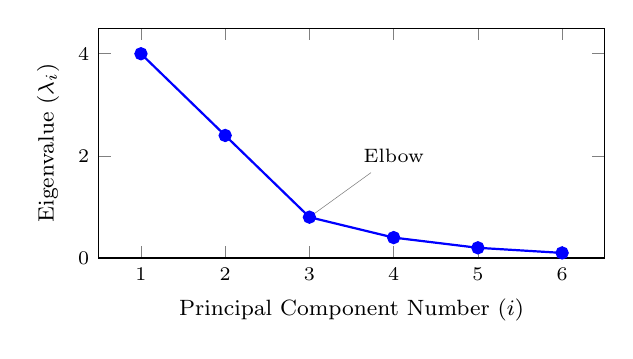
\begin{tikzpicture}
        \begin{axis}[
            xlabel={Principal Component Number ($i$)},
            ylabel={Eigenvalue ($\lambda_i$)},
            ymin=0, ymax=4.5,
            xmin=0.5, xmax=6.5,
            xtick={1,2,3,4,5,6},
            width=8cm, height=4.5cm,
            tick label style={font=\scriptsize},
            label style={font=\footnotesize}
        ]
        \addplot[thick, blue, mark=*] coordinates {
            (1, 4.0) (2, 2.4) (3, 0.8) (4, 0.4) (5, 0.2) (6, 0.1)
        };
        % Labeling the elbow point
        \node[coordinate, pin={[pin distance=0.8cm, font=\scriptsize]above right:{Elbow}}] at (axis cs:3,0.8) {};
        \end{axis}
    \end{tikzpicture}
    \end{center}
\end{frame}

\begin{frame}
   \frametitle{Sample principal components based on standardized data}
   \begin{itemize}
      \item Replace $S$ by $R$, the sample correlation matrix.
   \end{itemize}
\end{frame}

% \begin{frame}
%    \frametitle{Application of PCA}
%    \begin{center}
%       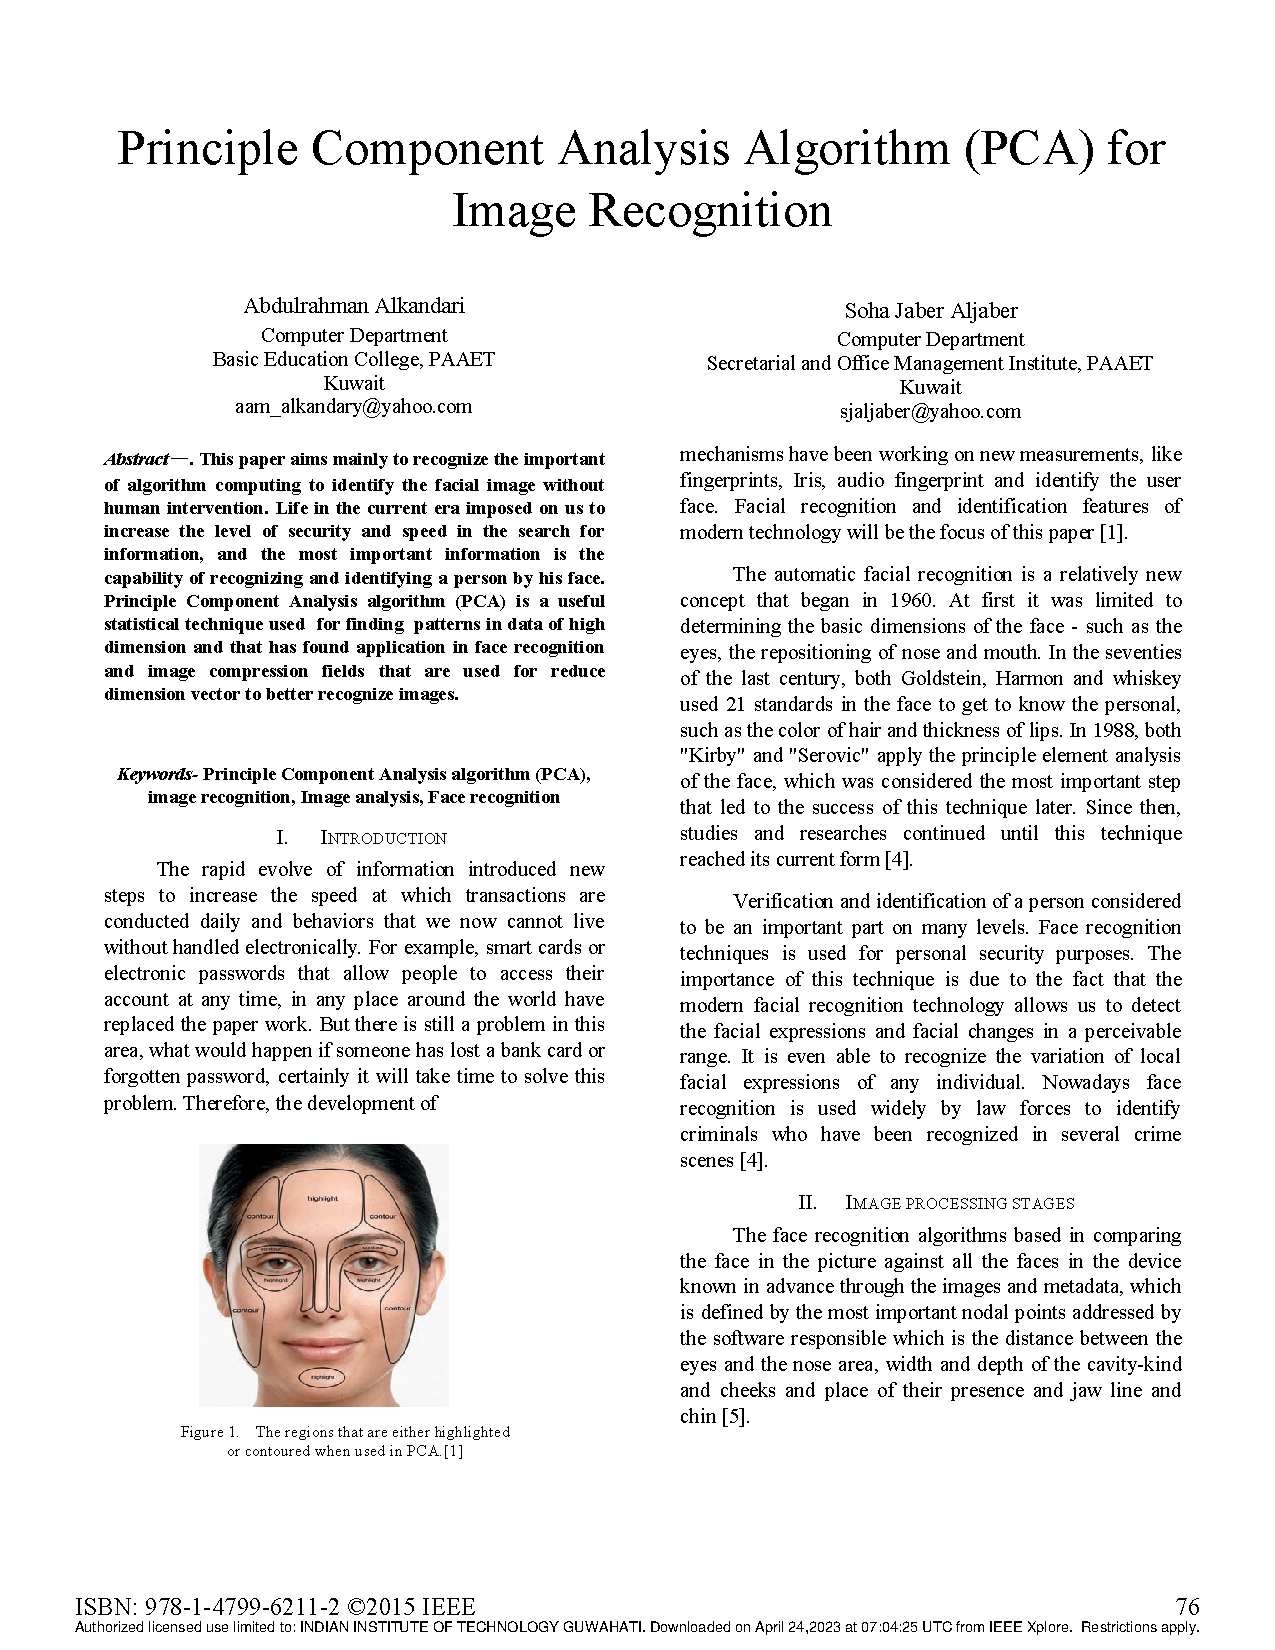
\includegraphics[page=1, trim=1cm 3cm 10cm 19cm, scale=1, width=13cm,
%       height=5cm, clip=true]{MVA-Principle_Component_Analysis_algorithm_PCA_for_image_recognition.pdf}
%    \end{center}
%    \vspace{0.05cm}
%
%    \begin{itemize}
%       \item Reference: Alkandari, A., \& Aljaber, S. J. (2015, April). Principle
%          Component Analysis algorithm (PCA) for image recognition. In 2015
%          Second International Conference on Computing Technology and Information
%          Management (ICCTIM) (pp. 76-80). IEEE.
%    \end{itemize}
% \end{frame}
%
% \begin{frame}
%    \frametitle{Application of PCA}
%    \begin{minipage}[c]{0.7\textwidth}
%    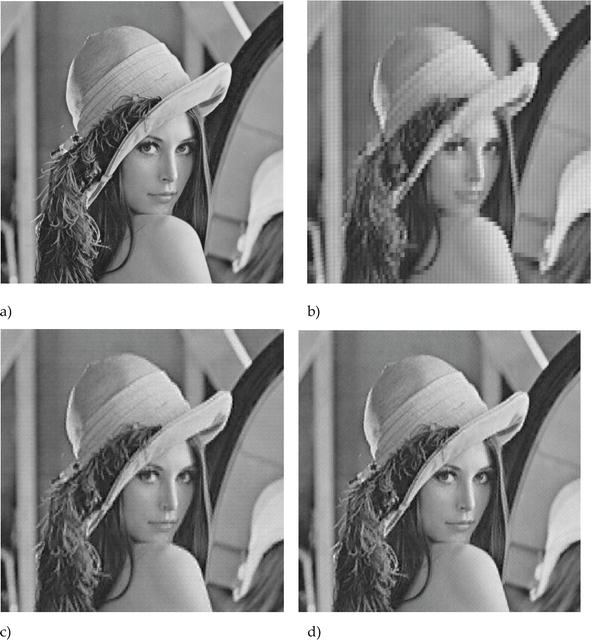
\includegraphics[ width=8cm, height=6cm]{MVA-F9.png}
%    \end{minipage}
%    \begin{minipage}[c]{0.25\textwidth}
%       (a) Original image.\\[1mm]
%       (b) Compression with two components.\\[1mm]
%       (c) Compression with five components. \\[1mm]
%       (d) Compression with eight components.
%    \end{minipage}
%    \begin{itemize}
%       \item Reference: Hernandez, W., Mendez, A., \& Göksel, T. (2018).
%          Application of principal component analysis to image compression.
%          Statistics-Growing Data Sets and Growing Demand for Statistics.
%    \end{itemize}
% \end{frame}
%
% \begin{frame}
%    \frametitle{Application of PCA}
%    Did you spot the bias in AI?
% \end{frame}
%
% \begin{frame}
%    \frametitle{Indian Face}
%    \vspace{0.25cm} 
%    \includegraphics[page=6, trim=10.5cm 12cm 0cm 10.5cm, scale=1, width=13cm,
%    height=5cm, clip=true]{MVA-Face_Matching_in_Indian_Citizens_using_CNN.pdf}
%    \vspace{0.05cm}
%    \begin{itemize}
%       \item A. S and S. R. Joshi, "Face Matching in Indian Citizens using
%          CNN," 2021 Second International Conference on Electronics and
%          Sustainable Communication Systems (ICESC), Coimbatore, India, 2021,
%          pp. 1343-1349.
%    \end{itemize}
% \end{frame}

\end{document}
